\documentclass[14pt, a1paper, portrait, margin=0mm, innermargin=5mm, blockverticalspace=7mm, colspace=5mm, subcolspace=8mm]{tikzposter}
%\documentclass{tikzposter}
\usepackage{array}
\usepackage{graphicx}
\usepackage{makecell}
\usepackage{fontawesome}
\usepackage{multicol}

%\renewcommand{\BackgroundPicture}{%
%  \put(-14,0){
%    \parbox[b][1.05\paperheight]{1.04\paperwidth}{%
%      \centering %
%      
\includegraphics[width=60cm]{img/ODK_elected_logo.png}
%    }
%  }
%}

\definecolorstyle{STACCStyle}{%
  \definecolor{stablue}{cmyk}{1,0.68,0,0.12} % Pantone 287 blue
  \definecolor{stared}{cmyk}{0,0.91,0.76,0} % Pantone 185 red
  \definecolor{stayellow}{cmyk}{0,0,1,0} % Pantone Yellow
  \definecolor{stablack}{cmyk}{0,0,0,1}
%  % secondary colours
  \definecolor{stalightblue}{cmyk}{1,0,0,0}
  \definecolor{staorange}{cmyk}{0,0.48,1,0}
  \definecolor{stagreen}{cmyk}{0.69,0,1,0}
  \definecolor{stadarkgreen}{cmyk}{1,0,0.48,0.6}
  \definecolor{stapurple}{cmyk}{0.46,0.63,0,0}
  \definecolor{staburgundy}{cmyk}{0,1,0.6,0.37}
  \definecolor{stagrey}{cmyk}{0,0.02,0,0.68}
}{%
  % Background Colors
  \colorlet{backgroundcolor}{stablue}
  \colorlet{framecolor}{stablue}
  % Title Colors
  \colorlet{titlefgcolor}{stablue}
  \colorlet{titlebgcolor}{white}
  % Block Colors
  \colorlet{blocktitlebgcolor}{stablue}
  \colorlet{blocktitlefgcolor}{white}
  \colorlet{blockbodybgcolor}{white}
  \colorlet{blockbodyfgcolor}{black}
  % Innerblock Colors
  \colorlet{innerblocktitlebgcolor}{white}
  \colorlet{innerblocktitlefgcolor}{black}
  \colorlet{innerblockbodybgcolor}{stablue!30!white}
  \colorlet{innerblockbodyfgcolor}{black}
  % Note colors
  \colorlet{notefgcolor}{black}
  \colorlet{notebgcolor}{staburgundy!50!white}
  \colorlet{noteframecolor}{stagrey}
}

\usebackgroundstyle{Empty}
\usecolorstyle{STACCStyle}

\makeatletter
\settitle{ \vbox{
    \begin{tabular}{p{5cm}p{43cm}p{5cm}}
      \vspace{0pt}
      \@titlegraphic
      &
        \vspace{0pt}
        \makecell[l]{
        \color{titlefgcolor}
        {\bfseries \Huge \sc Open Digital Research Environment Toolkit}\\
      \medskip
      \vspace*{1cm}
      {\huge for the Advancement of Mathematics}\\
      \medskip
      \vspace{1cm}
      {\huge \texttt{http://opendreamkit.org}}
      } 
      &
        \vspace{0pt}
        
\includegraphics[height=7cm]{img/groups-st-andrews-post.png}\\
    \end{tabular}
}}

\setlength{\TP@visibletextwidth}{\textwidth-2\TP@innermargin}
\newlength{\mytitlewidth}
\setlength{\mytitlewidth}{\textwidth-2\TP@innermargin}

\makeatother

\title{OpenDreamKit}
\author{Markus Pfeiffer\\ \texttt{markus.pfeiffer@st-andrews.ac.uk}}
\institute{University of St Andrews}
\titlegraphic{
  
\includegraphics[height=7cm]{img/ODK_elected_logo.png}
 \hfill 
}

\begin{document}
\maketitle[width=\mytitlewidth]
\block[titleinnersep=10pt]{Open Digital Research Environment Toolkit for the Advancement of Mathematics}{
  {\setlength{\columnsep}{30pt}%
  \begin{multicols*}{3}
    OpenDreamKit is a Horizon 2020 European Research Infrastructure project
    (\#676541) that will run for four years, starting from September 2015.

    \medskip

    It provides substantial funding to the open source computational (pure) mathematics
    ecosystem, in particular popular tools such as \texttt{GAP} \texttt{LinBox},
    \texttt{MPIR}, \texttt{SageMath}, \texttt{Pari/GP}, \texttt{LMFDB}, \texttt{Singular},
    \texttt{MathHub}, and the \texttt{Jupyter} interactive computing environment.
    
    \medskip

    The success of these systems over the past decades bears witness to the
    power of collaborative open source development models, by users and for users,
    for delivering general purpose systems, targeting a large public
    (researchers, teachers, engineers, amateurs, \ldots).
    
    \medskip

    We address some critical long term issues, in particular on the technical
    side, in order to boost the productivity and lower the entry barrier:
    \begin{itemize}
    \item Streamline access, distribution, portability on a wide range of
      platforms, including HPC and Cloud services.
    \item Improve user interfaces, in particular in the promising area of
      collaborative workspaces.
    \item Lower barriers between research communities and promote dissemination.
      For example, we want to make it easy for a specialist of scientific
      computing to use tools from pure mathematics, and vice versa; bring together
      the developers communities to promote tighter collaboration and symbiosis,
      accelerate joint development, and share best practices.
    \item Outsource as much of the development as possible to larger communities to
      focus on our core specialty: the implementation of mathematical algorithms
      and databases.
    \end{itemize}
 
    \medskip

    The project currently has 18 sites, and about 60 active researchers and software
    developers across Europe.
  \end{multicols*}}
}
\begin{columns}
  \column{0.666}
  \block[titleinnersep=10pt]{Maths in the Middle}{%
    \begin{multicols*}{2}
    \emph{Mathematics} is the common language which should be used
    to interface mathematical software. 

    \medskip
        
    \texttt{MMT} (Meta-Meta-Theory, Meta-Meta-Tool) is a highly flexible formal
    system striking a balance between `mathematical prose' and strict
    machine-checkable formalisation.
        
    \begin{tikzfigure}[Group Theory in MMT]
      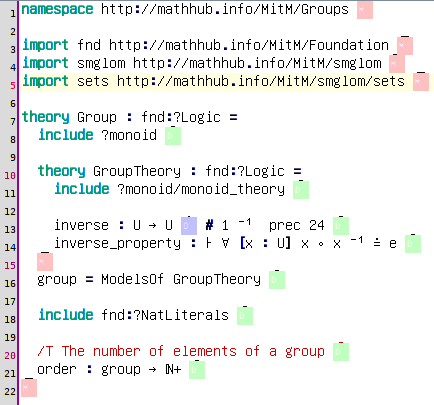
\includegraphics[width=12cm]{img/jedit-demo.png}
    \end{tikzfigure}
        
    We use \texttt{MMT} to describe \emph{semantic interfaces} to
    mathematical software packages, such as \texttt{GAP},
    \texttt{Sage}, \texttt{Singular}, databases such as \texttt{LMFDB} or
    the \texttt{ATLAS}, or databases of mathematical papers,
    such as the \texttt{arXiv}.
    
    The open interoperability standard \emph{Maths in the Middle} is built
    on these semantic descriptions, encoded in \texttt{OMDoc}, an extension
    to \texttt{OpenMath} and \texttt{MathML}, XML formats to represent
    mathematical knowledge.
        
    \begin{tikzfigure}[Maths in the Middle]
      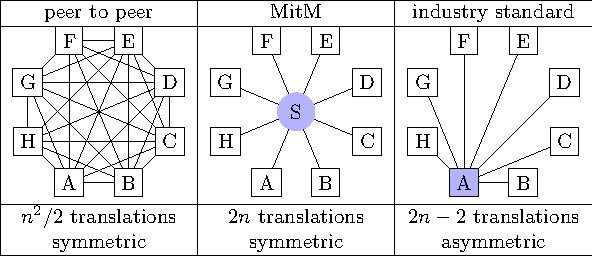
\includegraphics[width=12cm]{tikz/three-graphs.pdf}
    \end{tikzfigure}
    
    This lowers workload for implementors of mathematical software, enabling
    access to a large pool of external resources.

    \medskip
    
    Future plans include generating highly efficient interfaces with low
    computational overhead.
    \end{multicols*}
  }
  \block[titleinnersep=10pt]{MitM Usecases}{%
    \begin{multicols*}{2}
      Search mathematical texts for formulæ  \emph{structurally}:
      searching for $x^2 + y^2 = z^2$ will also yield results containing $a^2 + b^2 =
      c^2$.

      \medskip

      Search \texttt{OEIS} for formulæ and sequences, creating objects in the CAS
      of choice to do further computation.
      
      \medskip

      Query \texttt{LMFDB} from \texttt{GAP} for a Galois group,
      yielding a \texttt{GAP} group object that can be used in computations,
      for example to find out whether it is soluble.
      
      \medskip

      Explore the knowledge contained in and structure of \texttt{GAP}: types,
      relations, code. This can be done online, or through \texttt{MMT}. We make
      use of this information in the development of \texttt{GAP}.
    
%    \begin{tikzfigure}
%      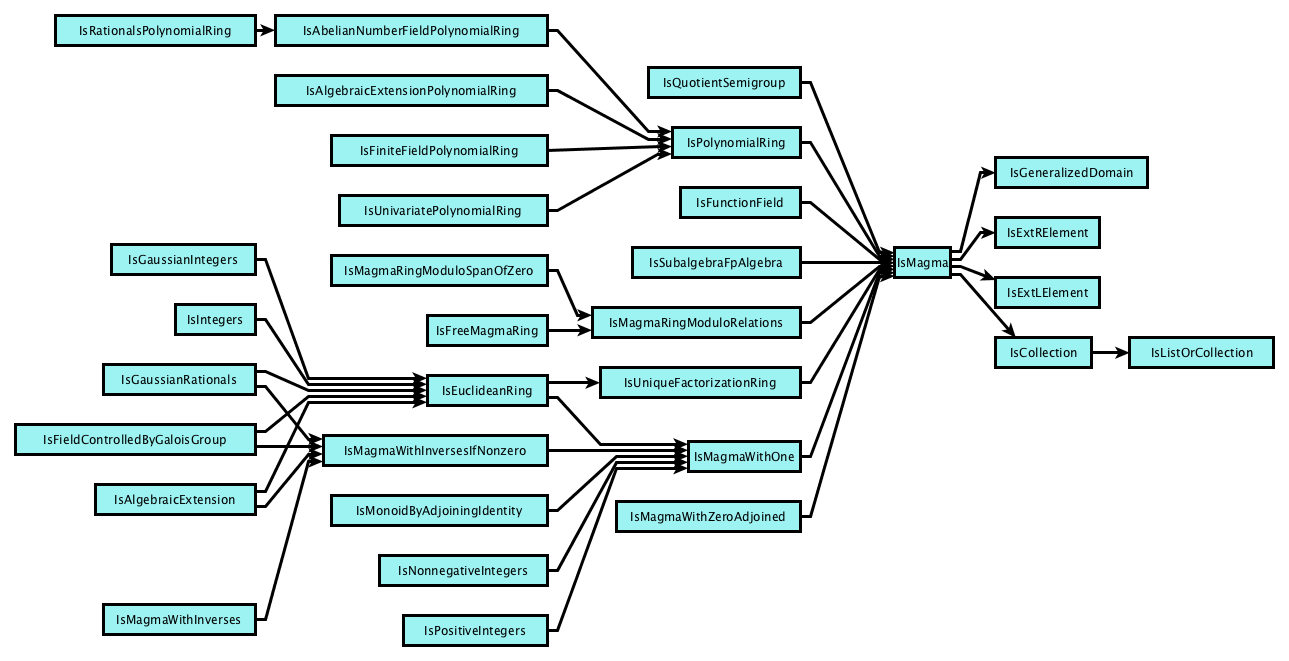
\includegraphics[width=12cm]{img/gap-ismagma.png}
%    \end{tikzfigure}
    
      \begin{tikzfigure}[GAP Theory Graph for \texttt{grp}]
        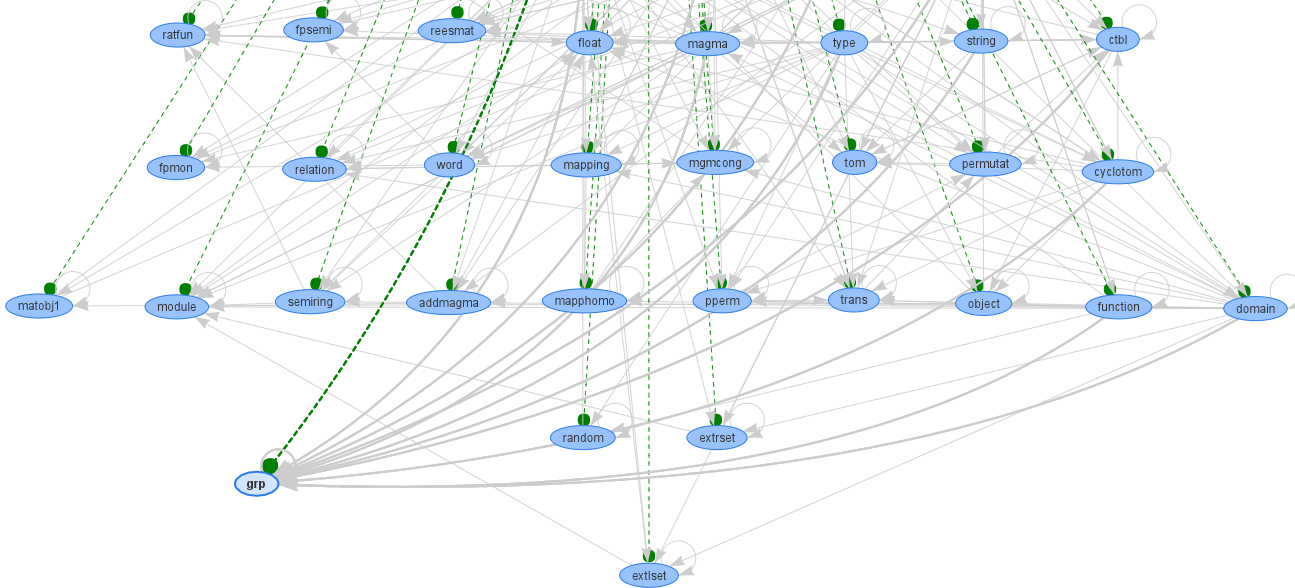
\includegraphics[width=12cm]{img/mmt-theorygraph-2.png}
      \end{tikzfigure}

      \begin{tikzfigure}[Browsing the GAP Type Export]
        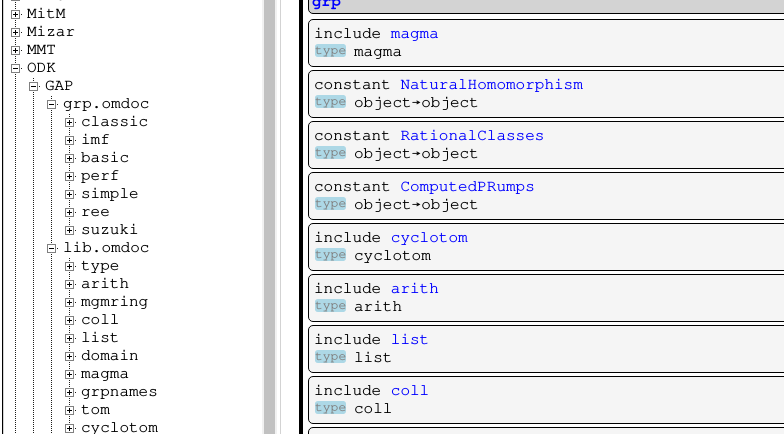
\includegraphics[width=15cm]{img/MMT-demo-2.png}
      \end{tikzfigure}

      \medskip

      Near future: Efficiently compute with group actions defined in
      \texttt{GAP} on polynomials defined in \texttt{Singular} through an
      automatically generated interface.

      \medskip

      \emph{Your usecase here: What would you want to do with Maths in the Middle?}

    \end{multicols*}
  }
  \column{0.333}
  \block[titleinnersep=10pt]{User Interfaces: Jupyter}{%
    Formerly known as \texttt{IPython}, \texttt{Jupyter} is a tool for writing
    interactive documents backed by a large selection of software packages.
    \texttt{JupyterHub} and \texttt{JupyterLab} allow institutional
    installations with ease.

    \medskip

    \texttt{Jupyter} has an excellent track record, an active community of
    contributors and is commercially backed by Bloomberg.

    \medskip

    We devloped a \texttt{GAP} interface for Jupyter, lowering the
    barrier to use \texttt{GAP} in research and teaching, making
    a web-based GUI for \texttt{GAP} a reality.

    \begin{tikzfigure}
      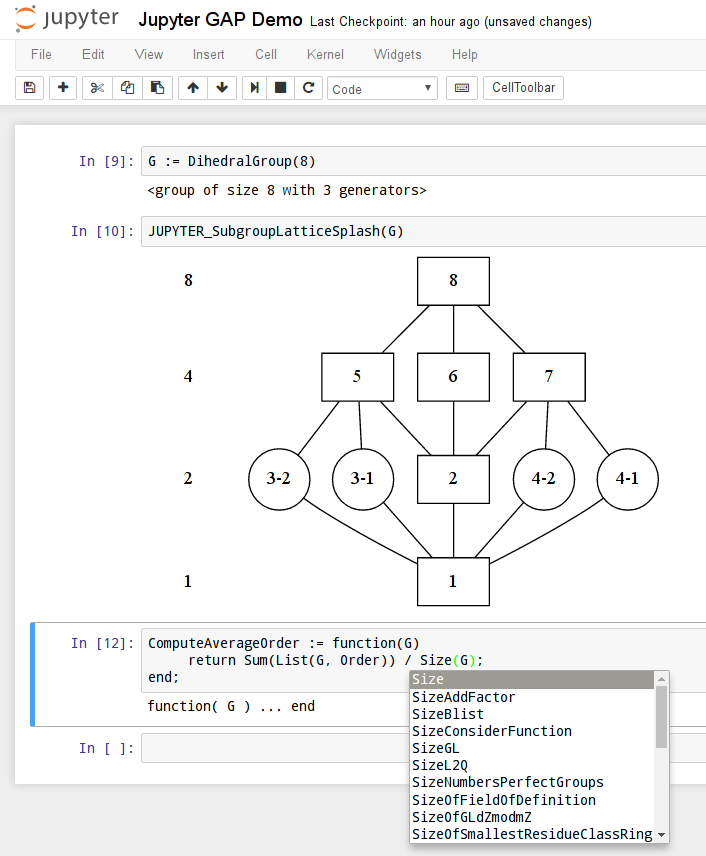
\includegraphics[width=15cm]{img/jupyter-demo-2.png}
    \end{tikzfigure}

    This interface is available through \texttt{PyPI}, the \texttt{Python}
    package index, and can be obtained by executing \texttt{pip install
      jupyter-kernel-gap} on many systems.

    \medskip

    We would like more users and contributors for this project and are looking
    forward to your input at \texttt{https://github.com/gap-packages/jupyter-kernel-gap}.
  } 
\end{columns}

%\begin{columns}
%  \block{High Performance Computation}{%
%    \begin{itemize}
%    \item Highly optimised multi-precision integer
%      libraries \texttt{MPIR}.
%    \item Highly optimised linear algebra
%    \item Improve the usablity and readiness of \texttt{HPC-GAP}
%    \item Develop and implement new parallel algorithms 
%    \end{itemize}
%  }
%\end{columns}

\block[titleinnersep=10pt]{Links}{%
  \begin{center}
    {\setlength{\tabcolsep}{1em}%
      \begin{tabular}{cccc}
        {\setlength{\tabcolsep}{0.2em}%
        \begin{tabular}{>{\centering\bfseries}m{2cm} >{\centering\arraybackslash}l}
          {\Huge \faHome} & \texttt{http://opendreamkit.org} \\ 
        \end{tabular}} &
        {\setlength{\tabcolsep}{0.2em}%
        \begin{tabular}{>{\centering\bfseries}m{2cm} >{\centering\arraybackslash}l}
          {\Huge @} & \texttt{contact@opendreamkit.org} \\  
        \end{tabular}} &
        {\setlength{\tabcolsep}{0.2em}%
        \begin{tabular}{>{\centering\bfseries}m{2cm} >{\centering\arraybackslash}l}
          {\Huge \faTwitter} & \texttt{@OpenDreamKit} \\ 
        \end{tabular}} &
        {\setlength{\tabcolsep}{0.2em}%
        \begin{tabular}{>{\centering\bfseries}m{2cm} >{\centering\arraybackslash}l}
          {\Huge \faGithub} & \texttt{https://github.com/OpenDreamKit} \\
        \end{tabular}} \\
      \end{tabular}}
    \medskip
    
    \begin{multicols*}{4}
      \begin{itemize}
      \setlength\itemsep{0.1em}
      \item[] \texttt{https://jupyter.org}
      \item[] \texttt{http://www.gap-system.org}
      \item[] \texttt{https://github.com/gap-system}
      \item[] \texttt{https://github.com/gap-packages}
      \item[] \texttt{https://www.singular.uni-kl.de/dox/html/}
      \item[] \texttt{https://sagemath.org}
      \item[] \texttt{https://cocalc.com}
      \item[] \texttt{http://mathhub.info}
      \item[] \texttt{http://mathhub.info/MitM}
      \item[] \texttt{https://uniformal.github.io}
      \item[] \texttt{https://openmath.github.io}
      \item[] \texttt{https://lmfdb.org}
      \item[] \texttt{https://arxiv.org}
      \end{itemize}
    \end{multicols*}
  \end{center}
}

\block{}{%
  \begin{tabular}{>{\centering\bfseries}m{6cm} >{\centering\arraybackslash}l}
    
\includegraphics[width=5cm]{img/Flag_of_Europe.png} & A project funded by the Horizon 2020 -- European Research Infrastructures Work Programme \\
  \end{tabular}
}
\end{document}

%%% Local Variables: 
%%% coding: utf-8
%%% mode: latex
%%% TeX-engine: XeTeX
%%% End: 